% APLAS 2021: Regular research papers should not exceed 18 pages in
% the Springer LNCS format(LaTeX template), including bibliography and
% figures.
% Lightweight double-blind: Author names and institutions must be
% omitted and References to the authors’ own related work should be in
% the third person 
%
\documentclass[runningheads]{llncs}
\pdfoutput=1
%\usepackage[english]{babel}
\usepackage[utf8]{inputenc}
\usepackage{amsmath}
\usepackage{amssymb}
%\usepackage{graphicx}
%\usepackage[colorinlistoftodos]{todonotes}
\usepackage{mathpartir}
\usepackage{graphicx}
%\usepackage{fixme}
\usepackage{xcolor}
\usepackage{hyperref}
\usepackage{listings}
\usepackage{titling}

%% structure
\newcommand{\Angle}[1]{\langle#1\rangle}

%% values
\newcommand\SUNIT{\textbf{()}}
\newcommand{\TRUE}{\textbf{True}}
\newcommand{\FALSE}{\textbf{False}}

%% names
\newcommand{\ALS}{\textbf{als}}
\newcommand{\PAK}{\textbf{pak}}
\newcommand{\PUK}{\textbf{puk}}
\newcommand{\PKH}{\textbf{pkh}}
\newcommand{\PUH}{\textbf{puh}}
\newcommand{\CODE}{\textbf{code}}
\newcommand{\BAL}{\textbf{bal}}
\newcommand{\COU}{\textbf{cou}}
\newcommand{\STORAGE}{\textbf{storage}}
\newcommand{\OP}{\textbf{op}}
\newcommand{\OPH}{\textbf{oph}}
\newcommand{\TIME}{\textbf{t}}
\newcommand{\CONTRACTORS}{\textbf{T}}
\newcommand{\PENDING}{\textbf{P}}
\newcommand{\ACCEPTED}{\textbf{A}}
\newcommand{\MANAGERS}{\textbf{K}}
%% operations
\newcommand{\TRANSFER}[5][\SUNIT]{\text{transfer $#2$ from $#3$ to $#4$ arg $#1$ fee $#5$}}
\newcommand{\ORIGINATE}[6]{\text{originate contract $#1$ transferring $#2$ from $#3$ running $#4$ init $#5$ fee $#6$}}
\newcommand{\NTEZ}{\textbf{n}}
\newcommand{\MTEZ}{\textbf{m}}
\newcommand{\ID}{\textbf{id}}
\newcommand\STRING{\textbf{s}}
%% queries
\newcommand{\QRY}{\textbf{qry}}
\newcommand{\GETBALANCE}[1]{\text{get balance for $#1$}}
\newcommand{\GETSTATUS}[1]{\text{get status for $#1$}}
\newcommand{\GETSTORAGE}[1]{\text{get contract storage $#1$}}
\newcommand{\GETCODE}[1]{\text{get code for $#1$}}
\newcommand{\GETPUBLICKEY}[1]{\text{get public key for $#1$}}
\newcommand{\GETCOUNTER}[1]{\text{get counter for $#1$}}

\newcommand{\ACCOUNTS}{\textbf{C}}
\newcommand{\OPERATIONS}{\textbf{O}}
\newcommand{\CONTRACTS}{\textbf{S}}

\newcommand{\NODE}{\textbf{N}}
\newcommand{\BLOCKCHAIN}{\textbf{B}}

%% functions
\newcommand{\CHECKACC}{\textup{checkAcc}}
\newcommand{\CHECKID}{\textup{checkId}}
\newcommand{\CHECKBAL}{\textup{checkBal}}
\newcommand{\CHECKCOU}{\textup{checkCou}}
\newcommand{\CHECKPUB}{\textup{checkPub}}
\newcommand{\UPDATECOU}{\textup{updateCou}}

\newcommand{\GENERATEOPH}{\textup{generateOph}}

%% transition relations
\newcommand{\NodeTrans}{\longrightarrow_N}
\newcommand{\SystemTrans}{\longrightarrow}

%\input{setup}

% ------------------- colors -------------------
\definecolor{darkgreen}{rgb}{0.0, 0.5, 0.0}
\definecolor{UniBlue}{RGB}{0, 74, 153}
\definecolor{UniRed}{RGB}{193, 0, 42}
\definecolor{UniGrey}{RGB}{154, 155, 156}
\definecolor{cverbbg}{gray}{0.93}

\newcommand{\todo}[1]{\textbf{\textcolor{red}{(TODO: #1)}}}

\begin{document}
%
\title{Assertion Contracts}
%
%\titlerunning{Abbreviated paper title}
% If the paper title is too long for the running head, you can set
% an abbreviated paper title here
%
%\author{Thi Thu Ha Doan\orcidID{0000-0001-7524-4497}\and Peter Thiemann\orcidID{0000-0002-9000-1239}}

%
%\authorrunning{Ha Doan, P. Thiemann}
% First names are abbreviated in the running head.
% If there are more than two authors, 'et al.' is used.
%
%\institute{University of Freiburg, Germany \\ \email{\{doanha,thiemann\}@informatik.uni-freiburg.de}
%}
%
\maketitle              % typeset the header of the contribution
%
\begin{abstract}
 \keywords{}
\end{abstract}

%
%
%
\section{Introduction}
\label{sec:introduction}
Every computation performed by a Smart Contract on the blockchain generates costs. Each
unit of computation and each unit of storage used by an algorithm must be paid for. To
avoid this cost, an application might perform some computation away from the blockchain
(i.e., off-chain) and submit the result as a parameter to a contract on the
blockchain. Typically, such a computation asserts certain properties of the 
submitted parameter. 

However, this approach raises the issue that on the one hand the contract should take
advantage of the offchain computation and assume that the submitted parameter has
these properties, but on the other hand, the off-chain computation might be wrong and
submit illegal parameters. So, we need a mechanism that checks the validity of the
assumptions before the contract starts executing.

As an example, consider a contract that takes a prime number as a parameter.
\begin{lstlisting}[numbers=none]
contract Example {
  function (int p) public {
    // assume p is prime
    ...
  }
}
\end{lstlisting}
This assumption can be expressed with an explicit assertion in predicate logic.
\begin{gather}\label{eq:5}
  (\forall n) (2 \le n \le \sqrt p) \Rightarrow (p \mathbin{\%} n) \ne 0
\end{gather}
To test the validity of this assumption requires a loop in the contract, but the test would take
$O(\sqrt p)$ time (assuming constant time for computing the remainder) and thus produce extra cost
linear in $\sqrt p$ accordingly. 
However, we could do better by recruiting the validators of the contract for a distributed
effort to find a counterexample. To this end, we consider the negation of the assertion.
\begin{gather}\label{eq:4}
  (\exists n) (2 \le n \le \sqrt p) \wedge (p \mathbin{\%} n) = 0
\end{gather}
This assertion can be checked pointwise by having each validator independently choose a
random $n$ fulfilling $2 \le n \le 
\sqrt p$ and checking whether $(p \mathbin{\%} n) = 0$. If the remainder is $0$, the
validator found a counterexample, posts its veto to the P2P net, and stops further
exection. Otherwise, it accepts $p$ knowing that other points will be checked by other
validators.

In this scenario, each validator only needs to be paid to generate a random number and
perform a division, which is a constant cost independent from $p$.

Of course, this validation is only probabilistic, so its effectiveness depends on the
number of validators. One could say that the community of validators implements a Bloom
filter for the set of primes: if a value $p$ is rejected it is certainly not a prime (because
there exists a counterexample); if a value $p$ is not rejected it is prime with a
probability that depends on $p$ and the number of validators. 

As another example, consider a contract that takes a sorted array of integers.
\begin{lstlisting}[numbers=none]
contract Sorted {
  function find (int[50] a, int v) public {
    // assume a is sorted
  }
}
\end{lstlisting}
The explicit assertion would be
\begin{gather}\label{eq:1}
  (\forall k) (0\le k <49) \Rightarrow a[k] \le a[k+1]
\end{gather}
While we can check this contract in $O(1)$ time, the constant factor is big! So we
consider its negation.
\begin{displaymath}
  (\exists k) (0\le k <49) \wedge a[k] > a[k+1]
\end{displaymath}
Again, we can have every validator generate a random number $k$. If the
condition is true for such $k$, then the validator found a counterexample for the sortedness
of the array. Otherwise, the validator relies on the other validators to check
different numbers.

To obtain an estimate of the number of validators needed to find a counterexample with
high probibility, 
let's assume the array is unsorted only at position $0$, the size of the array is $n$,
and the number of validators is $m$. Each validator independently has a probability of
$1/n$ to detect the problem and thus probability $\frac{n-1} n$ not to detect the
problem. Hence, if we assume that each $k$ is chosen independenty from a uniform distribution,
the probability that no validator checks at
position $0$ converges to $0$ as the number of validators approaches infinity.
\begin{displaymath}
  \lim_{m\to\infty}\frac{(n-1)^m}{n^m}
  = \lim_{m\to\infty} \left(\frac{n-1}{n}\right)^m
  = 0
\end{displaymath}

In Dafny (citation) \url{https://rise4fun.com/Dafny/tutorialcontent/guide#h29} you can
write
\begin{lstlisting}
forall j, k :: 0 <= j < k < a.Length ==> a[j] <= a[k]
\end{lstlisting}
to express that an array is sorted. This predicate is equivalent to the one given in
\eqref{eq:1}, but it might be more challenging to test. Its negation is
\begin{gather}
  \label{eq:2}
  (\exists j, k ) (0\le j< k < |a|) \wedge a[j] > a[k]
\end{gather}
So we'd have to generate two random numbers $j$ and $k$ such that the condition $0 \le
j < k < |a|$ is fulfilled.


Another condition that might be tested on an array is the heap condition
\begin{gather}
  \label{eq:3}
  (\forall i) (0 \le i < \lfloor|a|/2\rfloor) \Rightarrow a[i] \le a[2i+1] \wedge (2i+2
  < |a| \Rightarrow a[i] \le a[2i+2])
\end{gather}
\section{Primaries}
\label{sec:primaries}

\subsection{Smart Contract}
\label{subsec:smart-contract}

\subsection{Assertion Problem}
\label{subsec:problem}




\section{Distributed Assertion Protocol}
\label{sec:approach}
We propose an assertion verification approach for smart contracts. The idea underlying our approach is that the assertion is distributed to be verified by validators. During the distribution, each validator strives to find a counterexample for the assertion. Each of these validators then checks only a random point in the range of the parameter. Considering the example where a parameter $p$ is a prime number, the assertion in predicate logic for the parameter is 
\begin{gather}\label{eq:3a}
  (\forall n) (2 \le n \le \sqrt p) \Rightarrow (p \mathbin{\%} n) \ne 0
\end{gather}


\noindent and its negation form is 

\begin{gather}\label{eq:3b}
  (\exists n) (2 \le n \le \sqrt p) \wedge (p \mathbin{\%} n) = 0
\end{gather}

\noindent each validator independently choose a
random $n$ in the range $2 \le n \le 
\sqrt p$ and checking whether $(p \mathbin{\%} n) = 0$. If the remainder is $0$, the validator found a counterexample.

In our approach, there are three roles: 
\begin{itemize}
   \item the owner deploys and manages assertion contracts, 
   \item the callers invoke a assertion contract, and 
   \item the validators are involved in validating parameters. 
\end{itemize}

\noindent A caller submit a parameter that needs to be validated to the blockchain. The parameter is  then forwarded to all nodes as validators in the network, which then validate it. After the parameter is validated, the actual work that use the parameter is executed. 

Finding a counterexample for an assertion and announcing the result to the blockchain costs in terms of energy (computing power) and gas. There could be the case that it is very rare to find a counterexample, because a caller tries not to pass an unvalid parameter to the blockchain. In this case, we need to encourage all validators running the program to validate the assertion even though no counterexample may be found. Therefore, there are two way to reward validators in the form of cryptocurrency in order to motivate the validators to participate: (1) for a  counterexample found and (2) for a computational proof that proves that the validator actually run the program to find a counterfeit for the assertion, but none is found. If any of the validators finds a violation of the assertion, the final call to the actual work is aborted. 

An validator finds a counterexample for an assertion outside the chain. Therefore, validators interact with the on-chain contract to convey a found counterexample or computational proof via a function call. 

Since the parameter must be validated before the actual work can be performed, a caller first invokes an assertion function in the on-chain validation contract to pass the parameter for verification. After the parameter is verified, a work contract can be invoked to perform the actual task assuming that the parameter is valid. The work contract can be invoked by the on-chain validation contract only if certain conditions are met.

\paragraph{On-chain validation contract.} An on-chain validation contract must contain the following two functions:  

\begin{itemize}
\item the assertion function, where callers submit their parameters to be validated, which are then distributed to all validators. 
\item the on/off-chain assertion (validate function) to check and promote either a computational proof or a counterexample sent by the validators.
\end{itemize}


When a caller submits a parameter for validation, the parameter and associated information must be stored for the validation process. Since the parameter can be very large, we suggest storing only its hash. The hash is still sufficient to validate the validation process. The address of the caller should also be stored, and perhaps the timestamp indicating the approximate time the caller submitted the parameter. For each submission, there should be a corresponding record containing the associated data and validation status, such as the number of proofs received or the status if there is a counterexample. It could be the case that many parameters are submitted, then it may be useful to delete the record after the processing is completed with the parameter. There are two possible data structures for storing such records: map and array. 

For example, if we assume that a caller can submit only one parameter at a time, we can use a map that associates the caller's address with the parameter's hash and timestamp.

\begin{lstlisting}[numbers=none]

   struct Parameter {
        bytes32 p_hash;
        uint256 timestamp;
    }
    mapping (address => Parameter) public parameters;
\end{lstlisting}
 


\paragraph{On-chain work contract.}  The work contact can only be invoked by the on-chain validation contract after the parameter has been validated if no counterexample is found. The actual work is then performed with the passed parameter.

\paragraph{Off-chain validation contract.}
To check the validity of a parameter, each validator independently executes an off-chain validation contract that executes the on/off-chain assertion (the validate function), which is the same one used in the on-chain validation contract. The off-chain validation should be sent to all validators and executed outside the blockchain network. The on/off-chain assertion (the validate function) in the off-chain validation contract plays the main role in our approach. It contains the negation formulas of the assertion for parameters and takes a seed and a parameter as input. The seed is used to compute a random number to check the negation formulas. The result of the calculation can be a counterexample, an award computational proof, or a non-award computational proof.

A validator might try to run the off-chain validation contract many times to find either a counterexample or a computational proof. There could be many attempts before he receives an award. In the case of a non-award, the validator can run the code again with a different random number. If a counterexample or award is found, the validator passes the seed together with the parameter to the on-chain validation contract, which runs the same on/off-chain assertion and must end up with the same result as the counterexample or award.

\subsection{Managing on/off-chain contracts.}
All contracts are provided by their owner. The owner plays the main role in the design of the contracts. The owner deploy the on-chain validation contract and the work contract on the blockchain. 

The on/off-chain assertion and off-chain validation contract are stored off the blockchain and should be available to callers/validators upon request at any time. There are two ways to make them available to validators: (1) the codes are stored on a repository that callers/validators can access, or the owner can make it available to a caller/validator upon request, and (2) an owner/caller sends it to the network via messaging systems such as Waku in eutherum. The owners should send it to the network once they deploy the on-chain contracts, and in this case interested validators should store the code locally. In the same way, callers could also send it when they invoke an assertion function in the on-chain validation contract on the blockchain.
%\end{itemize}

\begin{figure}
\centering
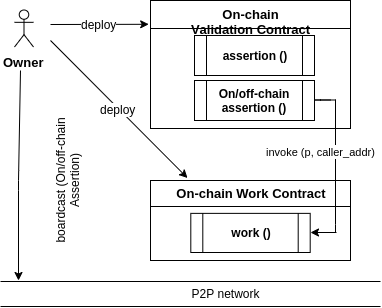
\includegraphics[scale=.8]{owner}
\caption{Managing on/off-chain assertion contracts.}
\end{figure}

\subsection{Interacting with the on-chain validation contract.}
A caller must first submit the parameter to an assertion function in the on-chain validation contract before it can be used in the work contract. The parameter is then distributed and validated by validators. The process of validating the parameter and invoking the work contract is transparent to the user. It is sufficient to store the hash of the parameter, and the parameter is transmitted when a validator invokes the on/off-chain assertion in the on-chain validation contract on the blockchain. Since the work contract is invoked by the on-chain validation contract, there should be a way to ensure that it is only invoked when the parameter is valid and certain conditions are met, e.g., when it has received a sufficient number of proofs. 

A caller may need to supply some tokens for validating the parameter and calling the work contract. 

In some cases where the validation process does not have a counterexample but does not meet some conditions, e.g., does not receive enough proofs from the validators, the owner has to do some tasks here to handle the refund since the functions in the smart contract are passive. Some time contracts could be used for this purpose.


\begin{figure}
\centering
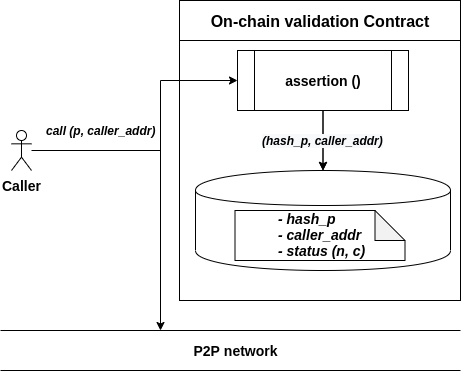
\includegraphics[scale=.6]{caller}
\caption{Submitting a parameter to the on-chain assertion contract.}
\end{figure}

\paragraph{Submitting a parameter.} A caller passes the parameter to be checked by calling an assertion function. The function then stores all necessary information, namely the hash of the parameter, the address of the caller, and possibly the timestamp, as if in a record. The parameter's record also contains initial information for monitoring the progress of the parameter's verification, e.g., how many computational proofs have been presented, whether a counterexample has been found, etc. This information is used to review a proof or counterexample presented by a validator, and to decide when a work contract can be called for that parameter. The caller may then send this information, along with the on/off-chain assertion and off-chain validation contract, to all validators via a messaging system.

\paragraph{Submitting of a computational proof/a counterexample.} After executing the off-chain validation contract, the validator may submit a computational proof or a counterexample to receive a reward. The submission contains the random number, the address of the validator, the parameter, and possibly other information. These are then used to calculate the seed, which then goes into the on/off-chain assertion along with the parameter. If the result is correct, there is an award to the validator and the record of the parameter in the storage accordingly is updated accordingly. When a computational proof is submitted and  certain requirements are met, the work contract is invoked. 

\subsection{Validating a parameter}
When a parameter is sent to a validator, the validator executes the off-chain validation contract, which includes an on/off-chain assertion, to find a counterexample. A validator interacts with the contract in two ways: it can announce a counterexample and submit a computational proof. If a counterexample is found, the validator submits it to the blockchain to receive a reward. Otherwise, a computational proof may be submitted. The computational proof is automatically generated when the on/off-chain assertion program is executed. The validator may need to clarify which parameter is being checked by submitting the parameter and the address of the caller, and possibly the timestamp. This information is then matched against the records in the storage. 

Since the on/off chain assertion is the same for every validator, we may need the address of the validator for each parameter to make the proof unique for each validator. A random number is combined with the validator's address to create a seed that is used to compute a random point in the parameter range to verify the validation of the parameter. This prevents the validator from copying a computational proof from others. With this information, a validator performs the off-chain validation contract, namely the on/off-chain assertion (validate function). There can be three different outcomes: a counterexample, an award, or a non-award. If it is a counterexample or an award, the validator passes the seed to the blockchain, i.e., it calls the on-chain validation contract on the chain, which then executes the same on/off-chain assertion. If the on-chain result is the same, the validator gets the reward. If the off-chain validation result is  non-award, the validator can rerun the off-chain validation. We could store these proofs information on the storage until the processing of the parameter is complete to prevent multiple submissions by a validator. 



\begin{figure}
\centering
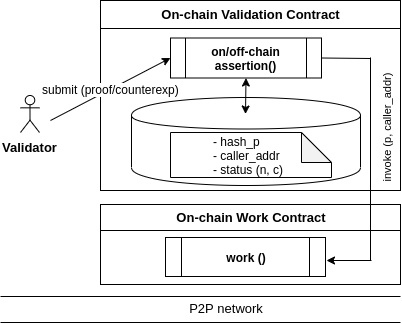
\includegraphics[scale=.8]{validator}
\caption{Submitting a proof/a counterexample.}
\end{figure}

\subsection{Calling a work function.}
The work function can only called by the on-chain validation contract once the parameter has been verified. Thus, the caller first passes its parameter to the assertion function and then waits a while to be sure that the parameter has been verified. The record corresponding to the parameter stored in the storage is updated when a proof or counterexample is presented. Some conditions must be met, e.g., after a certain amount of time has passed or enough evidence has been received from the validators.
If a validator submits the counterexample, the parameter is aborted from the validating process and the work contract is never called. Otherwise, the work contract is called when the computational proof is submitted and all conditions are met. 

 The on-chain validation contract calls the work contract with the current parameter and timestamp matched against the stored parameter hash and timestamp. They must match and satisfy some other conditions, such as a certain amount of time must have passed and no counterexample must be found. If all conditions are met, the actual work is done and the record of the parameter is deleted from memory to relieve the storage. If no record is found that matches the input data, the actual work with the input data is not performed. The work contract only allows the call from the on-chain validation contract.


\section{Domain Specification Language for Assertion}
We define a domain-specific high-level
language to express assertions.
\subsection{Assertion Grammar}
The syntax of this language is described in two versions by the grammars: prefix and infix. The parser currently supports the prefix notation and correct
operator precedences must be handled explicitly with parentheses. The syntax is inspired by OCaml and uses the same type notations as Michelson.

An assertion begins with the keyword entrypoint and a signature consisting of an optional tag, denoted by \%, followed by a parameter pattern. Parameter patterns are similar to patterns in OCaml — they are templates that match shapes of data structures and bind identifiers to the components of them. The given parameter pattern must match exactly the parameter type of the entrypoint it is associated with. The body of an assertion can
contain a nesting of quantifiers and conditions around exactly one assert expression, which tests a property. Conditions can be used to restrict the
quantification domains or to impose any other constraints. For completeness,
the existential quantifier is already included in the grammar, however the
current version of the pipeline will reject any assertions containing it.
How the assertions are associated with the respective entrypoint of the
parent contract, depends on the Smart Contract language. In the case of
Solidity, a tag that mirrors the function name is enough to link assertion and
entrypoint. In Michelson contracts, on the other hand, entrypoints can be
anonymous. Therefore, the assertions are linked to the entrypoints through
the tags, the parameter type or both. 

\subsubsection{Parameter patterns.}
Listing gives an overview of the parameter patterns supported in the assertion language.
\begin{lstlisting}[numbers=none]

< pattern > ::=
	| '_ '
	| nil
	| none
	| ( IDENT : < type >)
	| IDENT
	| ( pair < pattern > < pattern >)
	| ( left < pattern >)
	| ( right < pattern >)
	| ( cons < pattern > < pattern >)
	| ( some < pattern >)
   
\end{lstlisting}

\begin{lstlisting}[numbers=none]

( entrypoint % g ( pair ( cons a as ) _ ) ...)
\end{lstlisting}

AST

\begin{lstlisting}[numbers=none]

type ast =
{ entrypoint : string option * pattern ; body : assertion }

\end{lstlisting}

\subsection{Assertion Semantic}
A validator is trying to solve the following formula in a distributed form.

\begin{gather}
  \label{eq:2}
  \exists i \in D_{i}. P_{i}
\end{gather}

\noindent The verification attempt requires to search for $i$ in the domain $D$ such that $P_{i}$, called a counterexample. For each distributed trial, each validator chooses a random $i$ $\in$ $D$ and checks $P_{i}$. The formula can be extended to multiple domains $D_{i}$, ..., $D_{k}$.

\begin{gather}
  \label{eq:2}
\exists i \in D_{i}, \exists j \in D_{j}, ..., \exists k \in D_{k}. P_{i, j, ...,k}
\end{gather}

\subsubsection{Transformer. }
An assertion is formalized in the DSL. The formula is then transferred to its negation formula. 
\begin{gather}
  \label{eq:2}
\neg (\forall i \in D_{i}. P_{i}) \equiv \exists i \in D_{i}. \neg P_{i}
\end{gather}

\noindent Given an assertion
\begin{gather}
  \label{eq:2}
\forall i \in D_{i},  \forall j \in D_{j},  ..., \forall k \in D_{k}. P_{i, j, ...,k}
\end{gather}

\noindent it is then transformed to its negation, which is distributed to be verified by validators.

\begin{gather}
  \label{eq:2}
\exists i \in D_{i},  \exists j \in D_{j},  ..., \exists k \in D_{k}. \neg P_{i, j, ...,k}
\end{gather}

%(2) For nested quantifiers: a formula that may contain one (or more ''forall" qualifier) then all of these ''forall" quantifiers is converted to ''exist" and all ''exist" quantifiers are kept the same and negative the predicate.
%\begin{gather}
%  \label{eq:2}
%\forall i \in D_{i}, \exists j \in D_{j}, ..., \exists k \in D_{k}. (P_{i, j, ...,k})
%\end{gather}

%\begin{gather}
%  \label{eq:2}
%\exists i \in D_{i}, \exists j \in D_{j}, ..., \exists k \in D_{k}. \neg (P_{i, j, ...,k})
%\end{gather}


\subsection{Converter - Generating an On/off-chain Assertion} The main actor in our method is the on/off-chain assertion contract, which receives the parameter and a seed as input. The contract then generates a random number that is associated with a variable in the predicate. The result can be a counterexample, a computational proof with reward, or a computational proof without reward. A converter takes the AST of an assertion after the parser (or the AST for its negation after the transformer step) and returns the on/off-chain assertion contract written in Solidity (Michelson). To perform the conversion automatically, we restrict the semantics of the DSL. Variables are specified with \texttt{forall} quantifiers, which are then followed by \texttt{if} statements defining the range of the variable. For example, the following assertion specifies the parameter \texttt{a} of type \texttt{int} for the entrypoint \texttt{prime}. The next line defines the variable \texttt{a} of type \texttt{int} and its range is defined in the next \texttt{if} statement, namely [2 a/2]. Finally, the assertion is declared.

\begin{lstlisting}[numbers=none]

(entrypoint % prime (a : int)
   (forall (n : int)
         (if (and (ge 2 n) (le n (div a 2)))
              (assert (not (eq (mod a n) 0))))))
             
\end{lstlisting}



%, which then is checked   For the implementation of the current method, the syntax support any type of parameter, but the conversion supports the sematic for some typical types. Namely $i$ can be identified with a number. in deep the domain, $D$ should be able to associate with a natural number. For this end, a validator submits a seed that is then used to calculate $i$ that detects $P_{i}$. For example, arrays of any type or strings that is an array of characters. There could be several properties of natural numbers as primes, even, old, co-primes, square numbers, ..etc. for array $i$ could be used to detect the element of an array (or character of string). In some cases, when the formula is $\forall$ i $\in$ D. ($P_{i}$). The formula could be encoded an array of predicates. after an assertion is transferred to distributed form to be distributed. The most important in our approach is to design the validator contract that used both on-chain and off-chain computation. Our conversion converts an assertion to an on/off-chain assertion file that is used for validators to check a randomly chosen i. although our method and the assertion transformer works with all decide domain D. The convention will only work if the D is related to a natural number. 
\subsubsection{Detecting the range.} Assumes that the range of a variable is 
\begin{displaymath}
r = [a, b] \land (b-a) > 0
\end{displaymath}

\noindent and a seed $s$, then the random number in the range [a, b] can be generate by 

\begin{displaymath}
n = (s\mod(b - a)) + a.
\end{displaymath}


\noindent For the above assertion, we have  
\begin{displaymath}
r = [2 , a / 2] \land (a / 2 - 2) >= 0. 
\end{displaymath}

\noindent Given a random seed s, the $n$ $\in$ [2 , a / 2] could be generate by $s$.

\begin{gather}
n = (s\mod (a / 2 - 2)) + 2.
\end{gather}

\subsubsection{Calculating a valid hash.} a computational proof is based on Proof of work (as Bitcoin). Each computation calculates a hash based on its running the check of the predicate and then compare it with the target hash. The calculation has to be unique for each run to prevent copying of other validators or run a quick independent program to find a valid hash. To this end, we include the seed and the calculation of the predicate components to the hash. In this case, these above bad internal force can not be successful. A predicate is composed of the primitives with the following operations (\texttt{gt, lt, ge, le, or, xor, and, eq, neq, neg, not}). The operations are composed of one or more expressions. These expressions are then used to calculate the hash.

For example, given the predicate 

\begin{lstlisting}[numbers=none]
not (eq (mod a n) 0)
\end{lstlisting}

\noindent The expression \texttt{(mod a n)} is the used to calculate the hash.

The Converter generate a on/off-chain assertion program in Solidity as the follows.

\begin{lstlisting}[numbers=none]

pragma solidity >=0.7.0 <0.9.0;

/**
 * On/off-chain assertion contract 
 * to check counterexamples/computational proofs
 */
contract Validator{

    /**
    * The difficulty for a computational proof
    */
    uint diff = 1;
    uint public target = 2 ** (256 - diff); 

    /**
    * The result: 0 = non-award, 1 = proof, 2 = counterexample
    */

    function validate(uint p, uint seed) 
    public view returns (uint) {
        uint range = p / 2 - 2; 
        uint r = seed % range + 2;
        uint cal = p % r;

        uint result = 0; // an non-award computational proof 
        if (cal == 0)  
            result = 2; // a counterexample
        else 
            {
                uint result_target = 
                    uint (keccak256(abi.encodePacked(seed, cal)));
                if (result_target <= target) 
                    result = 1; // a computational proof    
            }
        return result;           
    }
}

\end{lstlisting}

For sorted array

\begin{lstlisting}[numbers=none]

(entrypoint % array (a : (list int))
   (forall (n : int)
      (forall (m : int)
         (if (and (ge n 1) (le n (size a)))
            (if (and (ge m 0) (lt m n))
                  (assert (le (nth a n) (nth a m))))))))
                  
\end{lstlisting}

\noindent We have:

$r_{n}$ = [1, size a] with (size a - 1 $>$ 0)

$r_{m}$ = [0, n] with (n - 0 $>$ 0)

\begin{lstlisting}[numbers=none]

pragma solidity >=0.7.0 <0.9.0;

/**
 * On/off-chain assertion contract 
 * to check counterexamples/computational proofs
 */
contract Validator{

    /**
    * The difficulty for a computational proof
    */
    uint diff = 1;
    uint public target = 2 ** (256 - diff); 

    /**
    * The result: 0 = non-award, 1 = proof, 2 = counterexample
    */

    function validate(uint[] memory p, uint seed)
    public view returns (uint) {
        uint range_1 = p.length - 1; 
        require(range_1 > 0, "invalid range");
        uint n = seed_i % range_1 + 1;
        uint range_2 = n;
        require(range_2 > 0, "invalid range");
        uint m = seed_j % range_2 ;
        
        uint cal_1 = p[m];
        uint cal_2 = p[n];

        uint result = 0; // an non-award computational proof 
        if (cal_1 > cal_2)  
            result = 2; // a counterexample
        else 
            {
            uint result_target = 
                 int (keccak256(abi.encodePacked(seed, cal_1, cal_2)));
            if (result_target <= target) 
                result = 1; // a computational proof      
        }             
        return result;           
    }
}

\end{lstlisting}

For a heap

\begin{lstlisting}[numbers=none]

(entrypoint % heap (a : (list int))
   (forall (n : int)
         (if (and (ge n 1) (le n (size a)))
                  (assert (lt (nth a n) (nth a (div (sub n 1) 2)))))))
\end{lstlisting}


\noindent We have:

$r$ = [1, size a] with (size a - 1 $>$ 0)


\begin{lstlisting}[numbers=none]
pragma solidity >=0.7.0 <0.9.0;

/**
 * Validator Contract
 * Check a counterexample/computational proof
 */
contract Validator{

    /**
    * The difficulty for a computational proof
    */
    uint diff = 1;
    uint public target = 2 ** (256 - diff); 

    /**
    * Check a counterexample/ computational proof
    * The result from a validator
    * 0 = non-award, 1 = proof, 2 = counterexample
    */

    function validate(uint[10] memory p, uint seed) 
    public view returns (uint) {
        uint range = p.length; 
        uint k = seed % range + 1;

        uint cal_1 = p[k];
        uint cal_2 = p[(k - 1) / 2];

        uint result = 0; // an non-award computational proof 
        if (cal_1 < cal_2)  
            result = 2; // a counterexample
        else {
            uint result_target = 
                uint (keccak256(abi.encodePacked(seed, cal_1, cal_2)));
            if (result_target <= target) 
                result = 1; // a computational proof      
        }              
        return result;           
    }
}

\end{lstlisting}

Coprimes number

\begin{lstlisting}[numbers=none]
(entrypoint % coprimes (pair (a : int) (b : int))
   (forall (n : int)
         (if (and (ge 2 n) (le n (if (ge a b) a b)))
              (assert (not (and (eq (mod a n) 0) (eq (mod b n) 0)))))))
\end{lstlisting}


\noindent We have:

$r$ = [2, (if (a $>=$ b) a b)] with ((if ($a >= b$) a b) - 2 $>$ 0)


\begin{lstlisting}[numbers=none]

pragma solidity >=0.7.0 <0.9.0;

/**
 * On/off-chain assertion contract 
 * to check counterexamples/computational proofs
 */
contract Validator{

    /**
    * The difficulty for a computational proof
    */
    uint diff = 1;
    uint public target = 2 ** (256 - diff); 

    /**
    * The result: 0 = non-award, 1 = proof, 2 = counterexample
    */

    function validate(uint a, uint b, uint seed)
    public view returns (uint) {
        uint range;
        if (a >= b) { range = a - 2; }
        else {range = b - 2;}
        
        uint r = seed % range + 2;
        require(range != 0, "invalid range");

        uint cal_1 = a % r;
        uint cal_2 = b % r;

        uint result = 0; // an non-award computational proof 
        if ((cal_1 == 0) && (cal_2 == 0))  
            result = 2; // a counterexample
        else {
            uint result_target = 
                uint (keccak256(abi.encodePacked(seed, cal_1, cal_2)));
            if (result_target <= target) 
                result = 1; // a computational proof      
        }              
        return result;           
    }
}

\end{lstlisting}

\section{A Prototype Implementation}
\section{Cost Analysis}
\section{Related work}
\section{Conclusion}

\newpage
\addcontentsline{toc}{chapter}{Appendix}
\clearpage
\appendix

\section{Type Soundness}
\label{sec:type-soundness}

\begin{lemma}[Canonical forms]\label{lemma:canonical-forms}
  Given a set of local accounts $\ACCOUNTS$, a blockchain
  $\BLOCKCHAIN$, and a typed value $\JTypeExpr\cdot \VAL \TYPE$.
  \begin{itemize}
  \item If $\TYPE=\TPUH$, then $\VAL=\PUH$ and $\PUH \in \DOM
    (\BLOCKCHAIN.\CONTRACTORS)$.
  \item If $\TYPE = \TPUK$, then $\VAL=\PUK$ and $\exists\PAK$ such
    that $(\PAK, \PUK) \in \ACCOUNTS$.
  \item If $\TYPE = \TADDR$, then $\VAL$ is $\PUH$ or $\PUK$.
  \item If $\TYPE = \TCONTRACT\ \TYPE_p\ \TYPE_s$, then $\VAL=\PUH$
    and $\PUH \in \DOM (\BLOCKCHAIN.\CONTRACTORS)$ and
    $\BLOCKCHAIN.\CONTRACTORS (\PUH) = (\CODE, \TIME, \BAL, \STORAGE)$
    such that $      \JTypeCode \CODE{ \TPAIR\ \TYPE_p\ \TYPE_s}$ and
    $\JTypeValue \STORAGE { \TYPE_s}$.
  \item If $\TYPE = \TCODE\ \TYPE\ \TYPEU$, then $\VAL = \CODE$ and
    $\JTypeCode \CODE{\TPAIR\ \TYPE\ \TYPEU}$.
  \item If $\TYPE = \TOPH\ \TYPE\ \TYPEU$, then $\VAL = \OPH$ and
    $\OPH\in \DOM (\BLOCKCHAIN.\PENDING)$ and $\BLOCKCHAIN.\PENDING
    (\OPH) = \Angle{\OP, \TIME, \STATUS}$ where $\TYPE=\TYPEU=\TNO$ if
    $\OP$ is a transfer and $\TYPE=\TYPE_p\ne\TNO$, $\TYPEU=\TYPE_s\ne\TNO$ if $\OP
    = \ORIGINATE\NTEZ\PUK\CODE\STRING\MTEZ$ and $\JTypeCode\CODE{
      \TPAIR\ \TYPE_p\ \TYPE_s}$.
  \item If $\TYPE = \TSTATUS$, then $\VAL \in \{\STATUSPENDING , \STATUSINCLUDING (\INT),
    \STATUSTIMEOUT\}$.
  \item If $\TYPE = \TEXCEPTION$, then $\VAL \in \{\ERRPRG, \ERRBAL, \ERRCOUNT, \ERRFEE,
    \ERRPUK, \ERRPUH, \ERRARG, \ERRINIT \}$.
  \item If $\TYPE = \TTEZ$, then $\VAL = \NTEZ$, a token amount.
  \item If $\TYPE = \TNO$, then $\VAL$ can be any syntactic value.
  \item If $\TYPE = \TINT$, then $\VAL = \INT$.
  \item If $\TYPE = \TUNIT$, then $\VAL = \SUNIT$.
  \item If $\TYPE = \TBOOL$, then $\VAL \in \{ \TRUE, \FALSE\}$.
  \item If $\TYPE = \TSTRING$, then $\VAL = \STRING$, a string.
  \item If $\TYPE = \TYPE\to\TYPEU$, then $\VAL = \lambda
    \VARIABLE. \EXPR$. 
  \item If $\TYPE = \TPAIR\ \TYPE\ \TYPEU$, then $\VAL = (\VAL',
    \VAL'')$ where $\JTypeExpr\cdot {\VAL'}\TYPE$ and $\JTypeExpr\cdot
    {\VAL''}\TYPEU$ in context $\ACCOUNTS$ and $\BLOCKCHAIN$.
  \item If $\TYPE = \TLIST\ \TYPE$, then either $\VAL = \NIL$ or $\VAL
    = \CONS\ {\VAL'}\ {\VAL''}$ where $\JTypeExpr\cdot{\VAL'}\TYPE$
    and $\JTypeExpr\cdot{\VAL''}{\TLIST\ \TYPE}$ in context
    $\ACCOUNTS$ and $\BLOCKCHAIN$.
  \item If $\TYPE = \TSUM\ \TYPE\ \TYPEU$, then either $\VAL = \LEFT\
    \VAL'$ where $\JTypeExpr\cdot {\VAL'}\TYPE$ or $\VAL= \RIGHT\
    \VAL''$ where $\JTypeExpr\cdot {\VAL''}\TYPEU$ in context
    $\ACCOUNTS$ and $\BLOCKCHAIN$.
  \item If $\TYPE = \TOPTION\ \TYPE$, then $\VAL = \NONE$ or $\VAL =
    \SOME\ \VAL'$ where $\JTypeExpr\cdot {\VAL'}\TYPE$ in context
    $\ACCOUNTS$ and $\BLOCKCHAIN$.
  \end{itemize}
\end{lemma}

\begin{lemma}[Subterm replacement]\label{lemma:subterm-replacement}
  If $\JTypeExpr\cdot{ \EC\EXPR}\TYPE$,
  $\JTypeExpr\cdot\EXPR \TYPE'$, and
  $\JTypeExpr\cdot{\EXPR'} \TYPE'$, then
  $\JTypeExpr\cdot{ \EC{\EXPR'}}\TYPE$.
\end{lemma}
\begin{proof}
  Induction on evaluation context $\ECN$ making use of the fact that
  an evaluation context does not bind variables.
\end{proof}

\begin{lemma}[Preservation for expressions]\label{lemma:type-preservation-expressions}
  If $\JTypeExpr\cdot{ \EXPR}\TYPE$ and $\EXPR \ExprTrans \EXPR'$,
  then  $\JTypeExpr\cdot{ \EXPR'}\TYPE$.
\end{lemma}
\begin{proof}
  Standard result: type preservation for simply typed lambda calculus
  with pairs, sums, and exceptions. Uses
  Lemma~\ref{lemma:subterm-replacement} for reductions in evaluation
  context. See, for instance, Types in
  Programming Languages by Benjamin Pierce.
\end{proof}

\begin{lemma}[Preservation]
  If $\BLOCKCHAIN[\overline\NODE] \SystemTrans{} \BLOCKCHAIN'[\overline{\NODE'}]$ and
  $\JTypeConfig\Delta {\BLOCKCHAIN[\overline\NODE]}$, then there is some
  $\Delta' \supseteq \Delta$ such that
  $\JTypeConfig{\Delta'}{ \BLOCKCHAIN'[\overline{\NODE'}]}$.
\end{lemma}
\begin{proof}
  The proof is by induction on the reduction relation
  $\BLOCKCHAIN[\overline\NODE] \SystemTrans{}
  \BLOCKCHAIN'[\overline\NODE']$ and inversion of the typing
  judgments. We only consider the exemplary reductions shown in the
  paper. We mark all components that belong to the reductum with 
  $'$ as in $\NODE'$.

  From $\JTypeConfig\Delta {\BLOCKCHAIN[\overline\NODE]}$ we obtain
  \begin{gather}
    \label{eq:1}
    \JTypeBlockchain\Delta\BLOCKCHAIN
    \\\label{eq:2}
    \JTypeNode{\NODE_i}
  \end{gather}
  From~\eqref{eq:1} we obtain
  \begin{gather}
    \label{eq:3}
    \DOM (\Delta) = \DOM (\BLOCKCHAIN.\CONTRACTORS)
    \intertext{and $\forall\PUH\in\DOM (\Delta)$}\label{eq:4}
    \Delta (\PUH) = \TPAIR\ \TYPE_p\ \TYPE_s
    \\\label{eq:5}
    \JTypeCode{\BLOCKCHAIN.\CONTRACTORS (\PUH).\CODE} {\TPAIR\ \TYPE_p\ \TYPE_s}
    \\
    \JTypeValue{\BLOCKCHAIN.\CONTRACTORS (\PUH).\STORAGE}{ \TYPE_s}
  \end{gather}
  From~\eqref{eq:2} we obtain, if $\NODE_i = [\overline{\EXPR_i},
  \ACCOUNTS_i]$, 
  \begin{gather}
    \label{eq:6}
    \JTypeExpr\cdot{ \EXPR_{ij}}\TUNIT
  \end{gather}

  \textbf{Reduction }$  \inferrule[Config-Node]
  {\NODE_0 \NodeTrans \NODE_0'}
  { {\BLOCKCHAIN[\NODE_0 :: \overline\NODE]}
    \SystemTrans
    {\BLOCKCHAIN[\NODE_0' :: \overline\NODE]}}$.

  The only possible reduction here is $  \inferrule[Node-Eval]
  {
    \EXPR \ExprTrans \EXPR'
  }{
    [\EC\EXPR :: \EXPRS, \ACCOUNTS] \NodeTrans{}
    [\EC{\EXPR'} :: \EXPRS, \ACCOUNTS]
  }$.

  From~\eqref{eq:6}, we know that $\JTypeExpr\cdot{ \EXPR}\TUNIT$. By
  Lemma~\ref{lemma:type-preservation-expressions}, $\JTypeExpr\cdot{
    \EXPR'}\TUNIT$, the types of the $\EXPRS$ are not affected, hence
  $\JTypeNode{\NODE_0' = [\EC{\EXPR'} :: \EXPRS, \ACCOUNTS]}$. None of the other
  nodes changed, neither did $\BLOCKCHAIN$, so that
  $\JTypeConfig\Delta{{\BLOCKCHAIN[\NODE_0' :: \overline\NODE]}}$. 

  \clearpage
  \textbf{Reduction }$\inferrule[Config-System]{
    \NODE\|\BLOCKCHAIN \SystemTrans \NODE'\|\BLOCKCHAIN'
}{
    \BLOCKCHAIN[\NODE :: \overline{\NODE}] \SystemTrans
    \BLOCKCHAIN'[\NODE' :: \overline{\NODE}]
  }$.

  We need to consider the cases for $\SystemTrans$.

  \textbf{Subcase }$  \inferrule[Node-Inject]{
    \Angle{\PAK,\PUK} \in \ACCOUNTS \\
    \CHECKBAL (\MANAGERS, \PUK, \NTEZ, \MTEZ) \\
    \CHECKARG (\CONTRACTORS, \PUH, \PARAMETER) \\
    \CHECKCOU (\MANAGERS, \PUK) \\
    \CHECKPUH (\CONTRACTORS, \PUH) \\
    \CHECKGAS (\CONTRACTORS, \PUH, \PARAMETER, \MTEZ) \\
    \OPH = \GENERATEOPH (\OP, \TIME) \\
    \OP = \TRANSFER[\PARAMETER]\NTEZ\PUK{\PUH}\MTEZ    
  }{
    { [\EC\OP :: \EXPRS, \ACCOUNTS] \|
      [\PENDING, \MANAGERS, \CONTRACTORS, \TIME] } \SystemTrans \\
    { [\EC{\OPH}  :: \EXPRS, \ACCOUNTS] \|
      [ \OPH \mapsto \Angle{\OP, \TIME, \STATUSPENDING}
      ::\PENDING,
      \UPDATECOU(\MANAGERS, \PUK, \TRUE),
      \CONTRACTORS,
      \TIME]
    }
  }$.
  Here $\NODE = [\EC\OP :: \EXPRS, \ACCOUNTS]$. We first check type
  preservation for the expression part. There are two typing rules for
  the transfer
  $\OP$, but only the one for contract invocation applies as the other
  one requires $\JTypeExpr\cdot{\PUH}\TPUK$, which does not hold.

  % For a token transfer
  % \begin{gather}
  %   \label{eq:7}
  %       \inferrule{
  %     \JTypeExpr\TEnv{\NTEZ}\TTEZ \\
  %     \JTypeExpr\TEnv{\PUK}\TPUK \\
  %     \JTypeExpr\TEnv{\PUH}\TPUK \\
  %     % \JTypeExpr\TEnv{\EXPR_3}{\TCONTRACT\ \TUNIT} \\
  %     \JTypeExpr\TEnv{\PARAMETER}\TUNIT \\
  %     \JTypeExpr\TEnv{\MTEZ}\TTEZ }{
  %     \JTypeExpr\TEnv{\TRANSFER[\PARAMETER]{\NTEZ}{\PUK}{\PUH}{\MTEZ}}\TOPH\
  %     \TNO\ \TNO
  %   }
  % \end{gather}

  For a contract invocation (specialized to empty environment)
  \begin{gather}
    \label{eq:8}
        \inferrule{
      \JTypeExpr\cdot{\NTEZ}\TTEZ \\
      \JTypeExpr\cdot{\PUK}\TPUK \\
      \JTypeExpr\cdot{\PUH}\TCONTRACT\ \TYPE_p\ \TYPE_s \\
      \JTypeExpr\cdot{\PARAMETER}{\TYPE_p} \\
      \JTypeExpr\cdot{\MTEZ}\TTEZ }{
      \JTypeExpr\cdot{\TRANSFER[\PARAMETER]{\NTEZ}{\PUK}{\PUH}{\MTEZ}}{\TOPH\
      \TNO\ \TNO}
    }
  \end{gather}
  The canoncical forms lemma~\ref{lemma:canonical-forms} is parameterized over the accounts
  $\ACCOUNTS$ of the local node and the current contractors
  $\BLOCKCHAIN.\CONTRACTORS$. Hence, we know that the arguments are
  legal, which is also checked by the rule.

  The reduct returns an operation hash $\OPH$ at type $\TOPH\ \TNO\
  \TNO$, which places no restrictions on the context of $\OPH$.

  Moreover, $\Delta' = \Delta$ and $\CONTRACTORS' = \CONTRACTORS$ as
  no new contract is originated.

  We conclude with Lemma~\ref{lemma:subterm-replacement} and
  reapplying \TirName{Config-System}.

  \textbf{Subcase }$\inferrule[Contract-Yes]{
    \JTypeCode\CODE{\TPAIR\ \TYPE\ \TYPEU} \\
    \BLOCKCHAIN.\CONTRACTORS (\PUH) =  \Angle{\CODE, \tilde\TIME, \NTEZ', \STRING'}
    % 
  }{
    { [\EC{\CAST\PUH\TPUH{\TCONTRACT\ \TYPE}}  :: \EXPRS, \ACCOUNTS] \|
      \BLOCKCHAIN
    }
    \SystemTrans
    { [\EC{\PUH} :: \EXPRS, \ACCOUNTS] \|
      \BLOCKCHAIN
    }
  }$.

  Immediate using Lemma~\ref{lemma:canonical-forms} and
  Lemma~\ref{lemma:subterm-replacement}.

  \textbf{Subcase }$\inferrule[Contract-No]{
    % \ADDR \in \DOM (\BLOCKCHAIN.\MANAGERS) \Rightarrow \TYPE\ne\TUNIT \\
    \BLOCKCHAIN.\CONTRACTORS (\PUH) = \Angle{\CODE, \tilde\TIME,
      \NTEZ', \STRING'} \Rightarrow {}
    \JTypeCode\CODE{\TPAIR\ \TYPE'\ \TYPEU} \wedge \TYPE \ne \TYPE' \\
  }{
    { [\EC{\CAST\PUH\TPUH{\TCONTRACT\ \TYPE}}  :: \EXPRS, \ACCOUNTS] \|
      \BLOCKCHAIN
    }
    \SystemTrans
    { [\EC{\RAISE\ \ERRPRG} :: \EXPRS, \ACCOUNTS] \|
      \BLOCKCHAIN
    }
  }$.

  The typing rule for $\RAISE$ can return any type. Hence, this is
  immediate by Lemma~\ref{lemma:subterm-replacement}.

  \textbf{Subcase }$\inferrule[Block-Originate]{
    \Angle{\PAK,\PUK} \in \ACCOUNTS \\ \CHECKBAL (\MANAGERS, \PUK, \NTEZ, \MTEZ) \\
    \CHECKCOU (\MANAGERS, \PUK) \\
    \CHECKPRG (\CODE) \\
    \CHECKGAS (\CODE, \INIT, \NTEZ, \MTEZ)  \\
    \CHECKINIT (\CODE, \STRING) \\
    % \OPH = \GENERATEOPH(\PUK, \CODE, \STRING, \NTEZ, \MTEZ, \TIME)
    % \\
    \OPH = \GENERATEOPH(\OP, \TIME) \\
    \OP = \ORIGINATE\NTEZ\PUK\CODE\STRING\MTEZ }{ [\EC\OP :: \EXPRS,
    \ACCOUNTS
    ] \| [\PENDING, \MANAGERS, \CONTRACTORS, \TIME] \SystemTrans \\
    [\EC{\OPH} :: \EXPRS, \ACCOUNTS] \| [\OPH \mapsto \Angle{\OP,
      \TIME, \STATUSPENDING} ::\PENDING,
    \UPDATECOU(\MANAGERS,\PUK,\TRUE), \CONTRACTORS, \TIME] }$. 
  
  Suppose that $\JTypeCode\CODE {\TPAIR\ \TYPE_p\ \TYPE_s}$. Then
  $\JTypeExpr\cdot\OP{\TOPH\ \TYPE_p\ \TYPE_s}$. But this is the type
  of the $\OPH$ in the reductum as it points to $\OP$ in
  $\PENDING$. Hence, the result is immediate by
  Lemma~\ref{lemma:subterm-replacement}.

  % \textbf{Subcase }$    \inferrule[Block-Accept-Query]{
  %   \OP = \ORIGINATE\NTEZ\PUK\CODE\STRING\MTEZ \\
  %   \PENDING (\OPH) =  \Angle{\OP,
  %     \hat\TIME, \STATUSINCLUDING\ \tilde\TIME} \\
  %   \PUH = \GENERATEHASH (\CODE, \tilde\TIME)
  %   % \CONTRACTORS (\PUH) =  \Angle{\CODE, \tilde\TIME, \NTEZ', \STRING'}
  % }{
  %   [\EC{\GETCONTRACT\ \OPH}  :: \EXPRS, \ACCOUNTS] \| [\PENDING, \MANAGERS, \CONTRACTORS, \TIME]
  %   \SystemTrans 
  %   [\EC{ \PUH}  :: \EXPRS, \ACCOUNTS] \|  [\PENDING, \MANAGERS, \CONTRACTORS, \TIME]
  % }$.

  

  \textbf{Subcase }$\inferrule[Query-Balance-Implicit]{
    % \BLOCKCHAIN =
    % [\PENDING, \PUK \mapsto \Angle{\BAL, \COU} :: \MANAGERS,
    % \CONTRACTORS, \TIME]
    \BLOCKCHAIN.\MANAGERS (\PUK) = \Angle{\BAL,\COU}
  }{[\EC{\GETBALANCE\PUK} :: \EXPRS, \ACCOUNTS] \| \BLOCKCHAIN
    \SystemTrans\ [\EC{\BAL} ::\EXPRS, \ACCOUNTS] \| \BLOCKCHAIN} $.
  
  The reduction replaces $\GETBALANCE\PUK$ of type $\TTEZ$ by $\BAL$
  of the same type. Hence, the result is immediate by
  Lemma~\ref{lemma:subterm-replacement}.

  \textbf{Subcase }$\inferrule[Query-Balance-Fail]{ \PUK \notin \DOM
    (\BLOCKCHAIN.\MANAGERS) \ }{[\EC{\GETBALANCE\PUK} :: \EXPRS,
    \ACCOUNTS] \| \BLOCKCHAIN \SystemTrans {[\EC{\RAISE\ \ERRPUK}
      ::\EXPRS, \ACCOUNTS] \| \BLOCKCHAIN}}$.

  Immediate by Lemma~\ref{lemma:subterm-replacement} because $\RAISE$
  can have any type.
    
  \clearpage
  \textbf{Reduction }$\inferrule[Config-Block]
  {\BLOCKCHAIN \BlockTrans \BLOCKCHAIN'}
  { \BLOCKCHAIN[{\overline\NODE}]
    \SystemTrans
    \BLOCKCHAIN'[{\overline\NODE}]}$.

  We need to considere cases for $\BlockTrans$.

  \textbf{Subcase }$\inferrule[Block-Accept]{
    \OP = \TRANSFER[\PARAMETER]\NTEZ\PUK{\PUH}\MTEZ \\
    \TIME - \hat\TIME \le 60
  }{
    { 
      [\OPH \mapsto \Angle{\OP, \hat \TIME, \STATUSPENDING}
      ::\PENDING, \MANAGERS,
      \CONTRACTORS, \TIME]}
    \BlockTrans 
    {
      [\OPH \mapsto \Angle{\OP, \hat\TIME, \STATUSINCLUDING\ \TIME} :: \PENDING}, \\
    { \UPDATESUCC (\MANAGERS, \PUK, \NTEZ, \MTEZ), 
      \UPDATECONSTR (\CONTRACTORS, \PUH, \NTEZ, \PARAMETER), \TIME +1]
    }
  }$.

  No typing-related properties are affected.

  \textbf{Subcase }$\inferrule[Block-Originate-Accept]{
    \OP = \ORIGINATE\NTEZ\PUK\CODE\STRING\MTEZ \\
    \PUH = \GENERATEHASH(\CODE, \TIME) \\
    \TIME-\hat\TIME  \le 60
  }{
    [\OPH \mapsto \Angle{\OP, \hat\TIME, \STATUSPENDING} :: \PENDING, \MANAGERS, \CONTRACTORS, \TIME]
    \BlockTrans \\
    [\OPH \mapsto \Angle{\OP, \hat\TIME, \STATUSINCLUDING\ \TIME} :: \PENDING, \UPDATESUCC
    (\MANAGERS, \PUK, \NTEZ, \MTEZ),\\ \PUH \mapsto  \Angle{\CODE, \TIME, \NTEZ, \STRING} :: \CONTRACTORS, \TIME+1]
  }$.
  
  This reduction extends $\CONTRACTORS$ with a new entry for
  $\PUH$. To preserve typing, we need to extend $\Delta$ with the
  binding $\PUH : \TPAIR\ \TYPE_p\ \TYPE_s$ where $\JTypeCode\CODE
  {\TPAIR\ \TYPE_p\ \TYPE_s}$. The generated code pointer is obtained
  with a query operation via the operation hash $\OPH$, which is also
  connected to the parameter and storage types. 

  \textbf{Subcase }$  \inferrule[Block-Timeout]{
    \TIME-\hat\TIME > 60
  }{ 
    {[\OPH \mapsto \Angle{\OP, \hat \TIME, \STATUSPENDING}
     ::\PENDING, \MANAGERS,
      \CONTRACTORS, \TIME]}
    \BlockTrans \\
    { 
      [\OPH \mapsto \Angle{\OP, \hat \TIME, \STATUSTIMEOUT}
     :: \PENDING,  \UPDATECOU(\MANAGERS, \OP.\PUK, \FALSE),
      \CONTRACTORS, \TIME]}
  }$.

  No typing-related properties are affected.
\end{proof}

\clearpage
\begin{lemma}[Progress for expressions]\label{lemma:progress-expressions}
  If $\JTypeExpr\cdot{ \EXPR}\TYPE$, then either
  \begin{itemize}
  \item $\EXPR$ is a value,
  \item $\EXPR \ExprTrans \EXPR'$, or
  \item $\EXPR = \EC{\EXPR'}$ is a blockchain operation in an evaluation context:
    \begin{itemize}
    \item $\EXPR' = \TRANSFER[\PARAMETER]\NTEZ\PUK{\PUH}\MTEZ$;
    \item $\EXPR' = \ORIGINATE\NTEZ\PUK\CODE\INIT\MTEZ$;
    \item $\EXPR' = \QOP\ \VAL$;
    \item $\EXPR' = \CAST\VAL\TYPE\TYPEU$ where $\TYPEU \SubType \TYPE$.
    \end{itemize}
  \end{itemize}
\end{lemma}
\begin{proof}
  Standard result: progress for simply type lambda calculus with
  pairs, sums, and exceptions. Upcasts are resolved by identity
  reductions. The blockchain operations including downcasts are not
  handled by the $\ExprTrans$ relation. 
\end{proof}
\begin{lemma}[Progress]
  If $\JTypeConfig\Delta{\BLOCKCHAIN[\overline\NODE]}$, then either
  all expressions in all nodes are unit values or there is a
  configuration $\BLOCKCHAIN'[\overline\NODE']$ such that
  $\BLOCKCHAIN[\overline\NODE] \SystemTrans \BLOCKCHAIN'[\overline\NODE']$.
\end{lemma}
\begin{proof}
  From $\JTypeConfig\Delta {\BLOCKCHAIN[\overline\NODE]}$ we obtain
  \begin{gather}
    \label{eq:101}
    \JTypeBlockchain\Delta\BLOCKCHAIN
    \\\label{eq:102}
    \JTypeNode{\NODE_i}
  \end{gather}
  From~\eqref{eq:101} we obtain
  \begin{gather}
    \label{eq:103}
    \DOM (\Delta) = \DOM (\BLOCKCHAIN.\CONTRACTORS)
    \intertext{and $\forall\PUH\in\DOM (\Delta)$}\label{eq:4}
    \Delta (\PUH) = \TPAIR\ \TYPE_p\ \TYPE_s
    \\\label{eq:105}
    \JTypeCode{\BLOCKCHAIN.\CONTRACTORS (\PUH).\CODE} {\TPAIR\ \TYPE_p\ \TYPE_s}
    \\
    \JTypeValue{\BLOCKCHAIN.\CONTRACTORS (\PUH).\STORAGE}{ \TYPE_s}
  \end{gather}
  From~\eqref{eq:102} we obtain, if $\NODE_i = [\overline{\EXPR_i},
  \ACCOUNTS_i]$, 
  \begin{gather}
    \label{eq:106}
    \JTypeExpr\cdot{ \EXPR_{ij}}\TUNIT
  \end{gather}

  For each such $\EXPR_{ij}$, Lemma~\ref{lemma:progress-expressions}
  yields that either
  \begin{itemize}
  \item $\EXPR_{ij}$ is a value; as it has type $\TUNIT$, we obtain
    $\EXPR_{ij} = \SUNIT$ by Lemma~\ref{lemma:canonical-forms};
  \item $\EXPR_{ij} \ExprTrans \EXPR_{ij}'$, in which case the whole
    system makes a step; or
  \item $\EXPR_{ij} = \EC{\EXPR}$ where $\EXPR$ is a blockchain operation.
  \end{itemize}

  \textbf{Subcase } $\EXPR =
  \TRANSFER[\PARAMETER]\NTEZ\PUK{\PUH}\MTEZ$. In this case, the
  \TirName{Node-Inject} reduction is in principle enabled:
  \begin{mathpar}
    \inferrule[Node-Inject]{
      \Angle{\PAK,\PUK} \in \ACCOUNTS \\
      \CHECKBAL (\MANAGERS, \PUK, \NTEZ, \MTEZ) \\
      \CHECKARG (\CONTRACTORS, \PUH, \PARAMETER) \\
      \CHECKCOU (\MANAGERS, \PUK) \\
      \CHECKPUH (\CONTRACTORS, \PUH) \\
      \CHECKGAS (\CONTRACTORS, \PUH, \PARAMETER, \MTEZ) \\
      \OPH = \GENERATEOPH (\OP, \TIME) \\
      \OP = \TRANSFER[\PARAMETER]\NTEZ\PUK{\PUH}\MTEZ    
    }{
      { [\EC\OP :: \EXPRS, \ACCOUNTS] \|
        [\PENDING, \MANAGERS, \CONTRACTORS, \TIME] } \SystemTrans \\
      { [\EC{\OPH}  :: \EXPRS, \ACCOUNTS] \|
        [ \OPH \mapsto \Angle{\OP, \TIME, \STATUSPENDING}
        ::\PENDING,
        \UPDATECOU(\MANAGERS, \PUK, \TRUE),
        \CONTRACTORS,
        \TIME]
      }
    }
  \end{mathpar}
  Thanks to the canonical forms Lemma~\ref{lemma:canonical-forms}, we
  know that $\Angle{\PAK,\PUK} \in \ACCOUNTS$, $\CHECKARG
  (\CONTRACTORS, \PUH, \PARAMETER)$ holds, and $\CHECKPUH
  (\CONTRACTORS, \PUH)$ holds. If one of the remaining checks fails,
  then one of the \TirName{Node-Reject} transitions throws an
  exception, so the configuration steps in every case. 

  \textbf{Subcase } $\EXPR = \ORIGINATE\NTEZ\PUK\CODE\INIT\MTEZ$. In
  this case, the \TirName{Block-Originate} reduction is in principle
  enabled:
  \begin{mathpar}
    \inferrule[Block-Originate]{
      \Angle{\PAK,\PUK} \in \ACCOUNTS \\ \CHECKBAL (\MANAGERS, \PUK, \NTEZ, \MTEZ) \\
      \CHECKCOU (\MANAGERS, \PUK) \\
      \CHECKPRG (\CODE) \\
      \CHECKGAS (\CODE, \INIT, \NTEZ, \MTEZ)  \\
      \CHECKINIT (\CODE, \STRING) \\
      % \OPH = \GENERATEOPH(\PUK, \CODE, \STRING, \NTEZ, \MTEZ, \TIME)
      % \\
      \OPH = \GENERATEOPH(\OP, \TIME) \\
      \OP = \ORIGINATE\NTEZ\PUK\CODE\STRING\MTEZ }{ [\EC\OP :: \EXPRS,
      \ACCOUNTS
      ] \| [\PENDING, \MANAGERS, \CONTRACTORS, \TIME] \SystemTrans \\
      [\EC{\OPH} :: \EXPRS, \ACCOUNTS] \| [\OPH \mapsto \Angle{\OP,
        \TIME, \STATUSPENDING} ::\PENDING,
      \UPDATECOU(\MANAGERS,\PUK,\TRUE), \CONTRACTORS, \TIME] }
  \end{mathpar}
  Thanks to the canonical forms Lemma~\ref{lemma:canonical-forms}, we
  know that $\Angle{\PAK,\PUK} \in \ACCOUNTS$, $\CHECKPRG (\CODE)$ holds, and $\CHECKINIT
  (\CODE, \STRING)$ holds. If one of the remaining checks fails,
  then one of the \TirName{Node-Reject} transitions throws an
  exception, so the configuration steps in every case. 
  
  \textbf{Subcase } $\EXPR = \QOP\ \VAL$. If $\EXPR =
  \GETBALANCE\VAL$, then inversion tells us that $\JTypeExpr\cdot{
    \VAL}\TADDR$ and by canonical forms
  (Lemma~\ref{lemma:canonical-forms}), it must be that $\VAL$ has the
  form $\PUK$ or $\PUH$. In any case, the value is a meaningful
  address for the manager $\MANAGERS$. Depending on whether the
  address is in use, one of the reductions
  \TirName{Query-Balance-Implicit} or \TirName{Query-Balance-Fail} can
  execute. There are further analogous reductions handling the case where
  $\VAL=\PUH$ and we ask for the balance of a smart contract.

  Most queries behave like $\GETBALANCE\cdot$, except getting a
  contract handle from an operation hash:

  \textbf{Subcase }$\EXPR = \GETCONTRACT\VAL$. This query is somewhat
  special as it is handled with reduction
  \TirName{Block-Accept-Query}. By inversion and canonical forms
  (Lemma~\ref{lemma:canonical-forms}) we know that $\VAL = \OPH$ is a
  valid operation hash of type $\TCONTRACT\ \TYPE\ \TYPEU$ where
  $\TYPE\ne\TNO$ and $\TYPEU \ne\TNO$.

  However, this reduction is conditional on the state of the
  transaction; it requires the new contract to have status
  $\STATUSINCLUDED$. If the contract has status $\STATUSTIMEOUT$, then
  the query raises and exception, analogous to the
  \TirName{Query-Balance-Fail} reduction. If the contract has status
  $\STATUSPENDING$, then the expression is blocked, but the system can
  make a step using \TirName{Block-Originate-Accept} that changes the
  status from $\STATUSPENDING$ to $\STATUSINCLUDED$. Alternatively,
  \TirName{Block-Timeout} can make a step to change the status to
  $\STATUSTIMEOUT$. In any case, the system as a whole can make a reduction.

  \textbf{Subcase } $\EXPR = \CAST\VAL\TYPE\TYPEU$ where $\TYPEU \SubType \TYPE$.
  As an example, we consider the reductions \TirName{Contract-Yes} and
  \TirName{Contract-No}, where a cast is applied to a value of type
  $\TPUH$. By canonical forms, we know that the value has the
  form $\PUH \in \DOM (\BLOCKCHAIN.\CONTRACTORS)$. The code pointed to
  by this hash is checked at run time and results either in a $\PUH$
  at suitable contract type (-Yes reduction) or in raising an
  exception (-No reduction). 

\end{proof}


%%% Local Variables:
%%% mode: latex
%%% TeX-master: "paper"
%%% End:


\newpage
\bibliographystyle{splncs04}
\bibliography{bio}
\end{document}


